%%%%%%%%%%%%%%%%%%%%%%%%%%%%%%%%%%%%%%%%%
% Thin Sectioned Essay
% LaTeX Template
% Version 1.0 (3/8/13)
%
% This template has been downloaded from:
% http://www.LaTeXTemplates.com
%
% Original Author:
% Nicolas Diaz (nsdiaz@uc.cl) with extensive modifications by:
% Vel (vel@latextemplates.com)
%
% License:
% CC BY-NC-SA 3.0 (http://creativecommons.org/licenses/by-nc-sa/3.0/)
%
%%%%%%%%%%%%%%%%%%%%%%%%%%%%%%%%%%%%%%%%%

%----------------------------------------------------------------------------------------
%	PACKAGES AND OTHER DOCUMENT CONFIGURATIONS
%----------------------------------------------------------------------------------------

\documentclass[a4paper, 11pt]{article} % Font size (can be 10pt, 11pt or 12pt) and paper size (remove a4paper for US letter paper)

\usepackage[protrusion=true,expansion=true]{microtype} % Better typography
\usepackage{graphicx} % Required for including pictures
\usepackage{wrapfig} % Allows in-line images
\usepackage{booktabs}

\usepackage{mathpazo} % Use the Palatino font
\usepackage[T1]{fontenc} % Required for accented characters
\linespread{1.05} % Change line spacing here, Palatino benefits from a slight increase by default

\makeatletter
\renewcommand\@biblabel[1]{\textbf{#1.}} % Change the square brackets for each bibliography item from '[1]' to '1.'
\renewcommand{\@listI}{\itemsep=0pt} % Reduce the space between items in the itemize and enumerate environments and the bibliography

\renewcommand{\maketitle}{ % Customize the title - do not edit title and author name here, see the TITLE block below
\begin{flushright} % Right align
{\LARGE\@title} % Increase the font size of the title

\vspace{50pt} % Some vertical space between the title and author name

{\large\@author} % Author name
\\\@date % Date

\vspace{40pt} % Some vertical space between the author block and abstract
\end{flushright}
}

%----------------------------------------------------------------------------------------
%	TITLE
%----------------------------------------------------------------------------------------

\title{\textbf{Exploiting LED Rolling-Shutter Effect in Indoor Positioning System}\\ % Title
Modern Mobile Communications} % Subtitle

\author{\textsc{Yang Guang} % Author
\\{\textit{1140339072}}} % Institution

\date{\today} % Date

%----------------------------------------------------------------------------------------

\begin{document}

\maketitle % Print the title section

%----------------------------------------------------------------------------------------
%	ABSTRACT AND KEYWORDS
%----------------------------------------------------------------------------------------

%\renewcommand{\abstractname}{Summary} % Uncomment to change the name of the abstract to something else

\begin{abstract}
It has been very mature to locate one's position in the outdoors using GPS like satellite positioning systems in a relatively acceptable deviation. However, Indoor Positioning System(IPS), still cannot be available in modern indoor environment such as airport or grand shopping plazas due to several constrains. But IPS has been proved to be very useful in the perspective future by the industry. Although this topic has been researched in recent 10 years in many related methods, there are two key issues of hardware cost against accuracy that cannot make a good balance between one another. In this article, we first give some research on related works of indoor positioning system, mainly on five systems of RADAR[00], Centaur[12], Cricket[04], Ubicarse[14], and Luxapose[14], then we fuifill the detail implementation of Luxapose, one method exploits visible light communication to realize IPS and evaluate its performance on some key factors of accuracy and available limit distance.
\end{abstract}

\hspace*{3,6mm}\textit{Keywords:} IPS , AoA , Rolling Shutter, VLC % Keywords

\vspace{30pt} % Some vertical space between the abstract and first section

%----------------------------------------------------------------------------------------
%	ESSAY BODY
%----------------------------------------------------------------------------------------

\section*{1. Introduction}

 Smart devices with cameras and LEDs are abundant in today's environment. This abundance creates an untapped opportunity for using these devices for wireless communication. Meanwhile, even if localization technology based on GPS developed maturely, we find the inconvenience with indoor localizations in malls or airports, which in fact in great need of the technology support of indoor localization since the environment is complex. Indoor localization serves these situations, and it can detect a wireless user's gesture, movement, or can do location-based authentication. In this article we draws a novel way by exploiting the LED lights to realize this indoor localization problem. 

 

This report does some survey on existing indoor localization methods and introduces some representative works in section 2. In section 3 we explicit the major task of Luxapose, involving the working scenario and techniques we planned to utilize, then we give a detailed definition of the indoor localization with LED AoA algorithm. In section 4 we introduced how the system been built on different modules. In section 5 we make an evaluation on several key metrics of location distance and accuracy and look forward to some future work that are needed to be worked on.

%------------------------------------------------

\section*{2. Related Works}
Indoor localization has been worked on for years since its demand in industry is badly. We review four major representative work based on RF, acoustic, and MIMO techniques, the four main methods today in research of indoor localization. We analysis their defects to show the advancement in our work of Indoor Localization with LEDs.

\subsection*{2.1 RF-based Localization \cite{Radar00} \cite{Centaur12}}
WiFi-based indoor localization approaches have been the center of attention in the field of indoor localization, due to their low deployment cost, potential for reasonable accuracy and readiness to be applied to mobile devices. Existing WiFi-based solutions usually fall into one of two categories: fingerprint-based and model-based approaches. We introduce fingerprint-based method by the Radar system, and model-based by the Centaur system.

While these methods have been shown to achieve promising localization accuracy (below 10 meters at 90\% tile) under lab conditions, large-scale accurate indoor localization systems have yet to be developed. For example, given realworld fingerprint sampling conditions, the localization accuracy of existing approaches in large venues like shopping malls and airports can still be up to 25m at 90\% tile; similar results are reported by Google\cite{google}

\subsubsection*{2.1.1 RF-based Localization \cite{Radar00}}
The fingeprint-based solution fingerprints locations in the area pf interest and then searches for the best matching location.

The model-based solution trains a signal propagation model using training/calibration data then applies trilateration for localization. 

Radar first collects fingerprints from various known locations to build up a fingerprint database. It then determines the position of an incoming fingerprint by comparing it against all fingerprints in the database, an averages the locations of a few fingerprints nearest in signal space.

\begin{figure}[h]
	\centering 
	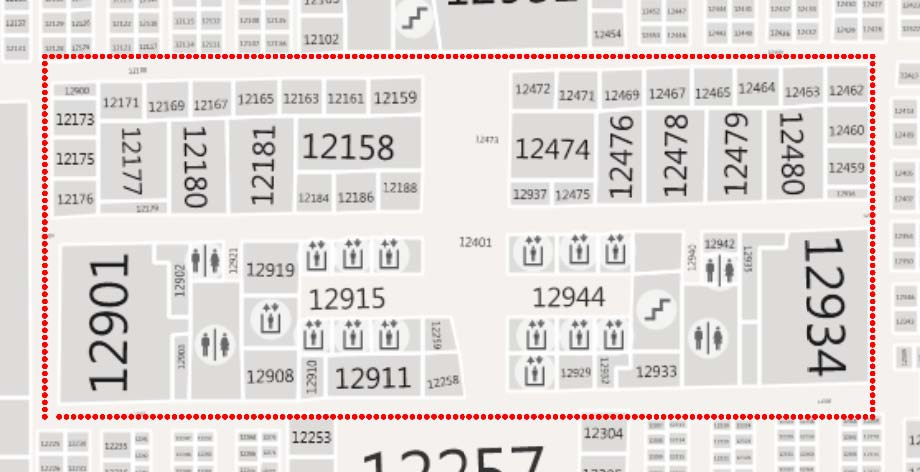
\includegraphics[width=0.8\linewidth]{Figure1.jpg}
	\caption{An office aera for data collection. Each red dot represents a sampling location. One fingerprint is collected for each location.\cite{Modellet14}}
	\label{fig:subfig}
\end{figure}

\subsubsection*{2.1.2 RF-based Localization \cite{Centaur12}}
Centaur adopts the log-distance path loss (LDPL) model and trains model parameters from fingerprints with known locations. Model parameters instead of fingerprints are stored in the location database. Trilateration or multilateration is applied to estimate the location for an incoming fingerprint.

Centaur and Radar are rooted at the irregularity of a \emph{radio map}, a map of signal strengths at different locations, and the ability to approximate the radio map from training data. The localization process is actually a process to find the best match(es) to a given fingerprint from the radio map and return the position of the best match(es). The better we can approximate the actual radio map, the better the localization accuracy that can be achieved.

When the training data are sparse, the radio map cannot be well approximated with few fingerprints. However, under the assumption of a radio propagation model, the radio map can be better approximated. The model requires only a few samples to train the model parameter. On the contrary, when the training data are dense, distances between fingerprints are close. Thus, direct use of the fingerprints can well approximate the radio map, whereas an oversimplified omni-model will lead to a high fitness error.\cite{Modellet14}

\subsection*{2.2 Acoustic-based Localization \cite{Cricket04}}
Some systems exploits the acoustic band into the field of indoor localization. The Cricket system \cite{Cricket04} use a difference of ultrasound and RF signal time-of-flight measurement technique to provide location. The system requires to establish several anchor points in the indoor environment, each point can publish RF packets and ultrasonic signals. The workflow presents as below: 

\begin{enumerate}
	\item Beacons publish information on an RF channel. With each RF advertisement, the beacon transmits a concurrent ultrasonic pulse.
	\item Listeners attached to devices and mobiles listen for RF signals, and upon receipt of the first few bits, listen for the corresponding ultrasonic pulse.
	\item Cricket exploits the difference of time-of-arrival of the paired signals to judge its distance with the Beacon source. By analysing different beacons, Cricket locate the listener's place with the help of trilateration or multilateration mathmatical methods.
\end{enumerate}

Cricket can reach high precise of several centimeters. However the drawback is its heavy hardware deployment requirement that limits its deployment.


\subsection*{2.3 MIMO-based Localization \cite{Ubicarse14}}
MIMO technology develops rapidly recently in RF communication field. By exploiting multiple antennas, one device can locate its place precisely with the aid of multiple APs in the environment. Ubicarse exploits the fact that today's tablets and smartphones have two or at most three antennas. This system make use of these antennas to form a MIMO system. However only two-antennas MIMO can't get a good localization output, so Ubicarse defines a rotate movement, that the user rotates the two-antennas MIMO to form a circular antenna array as shown in Figure 2, by the simulated antenna array the system can get a considerable improvement in precise of less than 30 centimeters.
\begin{figure}[h]
	\centering 
	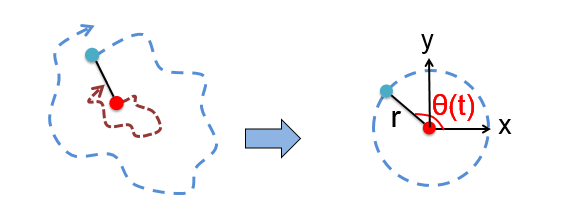
\includegraphics[width=0.8\linewidth]{Figure4.png}
	\caption{Virutual MIMO array of Ubicarse}
	\label{fig:subfig}
\end{figure}

%------------------------------------------------

\section*{3. Problem Definition and Algorithm of Luxapose}
Other systems such as Luxapose exploits the Visible Light Communication (VLC) technique. Luxapose use LED luminaries as visual light beacons. Landmarks are visible and distinguishable from each other. Location information is encoded by controllable frequencies. A phone receives these transmissions using its camera. By decoding the received signal, the phone get the location it lies.

Using LED luminaries has an obvirous advantange that it needs hardly additional devices besides the LED luminaries, which distributed everywhere in modern indoor buildings. It also needs smartphones with cameras which are ubiquitous in modern society. And it can reach a high accuracy of 0.1m, can be viewed as one of the most precise methods in the field of IPS. The table below specifically shows the performance of the surveyed five indoor positioning systems.

\begin{table}[htbp]	
	\centering 
	\begin{tabular}{lclclclclcl}
		\toprule
		Param & Radar & Centaur & Cricket & Ubicarse & Luxapose \\
		\midrule
		Reference & \cite{Radar00} & \cite{Centaur12} & \cite{Cricket04} & \cite{Ubicarse14} & \cite{Luxapose14}\\
		Position & 3-5m & 2-7m & 0.1m & 0.3m & 0.1m\\
		Method & FP & Model & DC & MIMO & AoA\\
		Database & YES & YES & YES & NO & NO\\
		\bottomrule
	\end{tabular}
	\caption{\label{tab:test}Performance of Surveyed IPS.FP, DC, AoA are FingerPrinting, Device Configuration, Angle-of-Arrival}
\end{table}


Luxapose consists of visible light beacons, smartphones with camera to take pictures, and a server that work together to determine the location of smartphone given its token pictures. For each beacon, it consists of a programmable microcontroller that controls LEDs to blink at specific frequencies that can broadcast its location information. For the smartphone camera, it needs to modify its camera parameters such as exposure time, ISO, in order to take high quality images that can reflect the beacon's rolling shutter effect. The server work with token pictures, and do a image processing pipeline to read frequency informations from the picture, then apply AoA(Angle-of-Arrival) algorithm to calculate the absolute location of the smartphone.

The main idea is AoA algorithm. AoA is a projection algorithm that can get the relative location of a given object with the aid of a picture of it. It needs three or more led beacons with known 3-D coordinates and these beacons can be located in an image captured by a smartphone, and they are visible and distinguishable from each other. Assuming that the camera geometry is known and the pixels onto which the beacons are projected is determined, we estimate the position and orientation of the smartphone with respect to the beacons' coordinate system through the geometry of similar triangles, using a variation on the well-known bearings-only robot localization and mapping problem\cite{AoA}.

In order to determine the corresponding relationship between beacons and transmitters on the image, we exploit the rolling shutter effect to find the pairing relationship. When capturing an image, most CMOS imagers expose one or more columns of pixels, but read out only one column at a time, sweeping across the image at a fixed scan rate to create a rolling shutter, as shown in Figure 3. When a rapidly modulated LED is captured with a CMOS imager, the result is a banding effect in the image in which some columns capture the LED when it is on and others when it is off. This effect is neither visible to the naked eye, nor in a photograph that uses an auto-exposure setting. However, the rolling shutter effect is visible when an image is captured using a short exposure time. And this is what we need to do with the module of an image capturer.

\begin{figure}[h]
	\centering 
	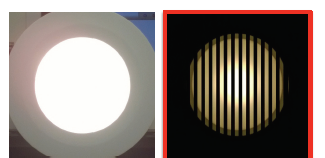
\includegraphics[width=0.8\linewidth]{Figure2.png}
	\caption{Rolling shutter effect}
	\label{fig:subfig}
\end{figure}

\section*{4. System Modules Implementation}
The system is implemented in four main modules. The four modules are presented below:
\begin{enumerate}
	\item Beacon Controller. It was implemented with Arduino DUE board. We presented five LEDs in one beacon for redundant.
	\item Camera. We use Lumia 1020 since it has an excellent performance in taking pictures with 4.1M pixels. We modified an open source WinPhone camera application \textit{Nokia Camera Explorer\cite{NCE}}. 
	\item Image Process Pipeline. It was deployed on the server with OpenCV, and its purpose is decoding the captured image, locate at least 3 transmitters, identify the frequency and apply them as input for AoA.
	\item AoA. Its inputs are from the image processing pipeline, and using several given parameters, we apply the AoA algorithm to calculate the location of the user.
\end{enumerate}

\subsection*{4.1 Beacon Controller}
We deploy five LED beacons in a 60cm*60cm rectangle place as in Figure 4, and we set the frequencies of the five beacons as 2000Hz, 2500Hz, 3000Hz, 3500Hz, 4000Hz, each with a coordinate of (-5,5,0), (5,5,0), (5,-5,0), (-5,-5,0) and (0,0,0). 
The frequency of each LED beacon is controlled using Arduino DUE board. Arduino is a programmable open-source hardware. We exploit its clock and use bit operation to produce the 5 kinds of different frequencies, and using a transistor with several limiting resistors to work as a relay to drive a 25V DC circuit of 5 led luminaries.
\begin{figure}[h]
	\centering 
	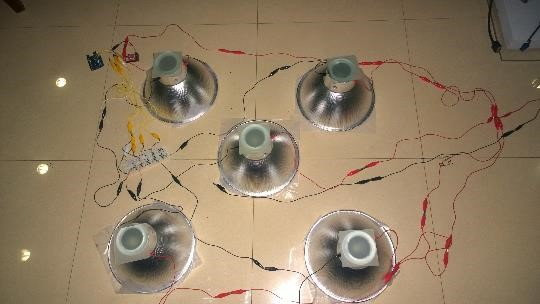
\includegraphics[width=0.8\linewidth]{Figure3.jpg}
	\caption{Rolling shutter effect}
	\label{fig:subfig}
\end{figure}

\subsection*{4.2 Camera}
We choose to use the Lumia 1020 as our image capture device since it gives an excellent camera and its API of camera setting parameters are given by Nokia which includes expose control of resolution, exposure time and film speed.

We modify the Nokia Camera Explorer\cite{NCE} to build our application.We augment the app to expose the full range of resolution and exposure settings, and we add a streaming picture mode that continuously takes images as fast as the hardware will allow. And finally we transfer captured images to the server for image processing and apply AoA algorithm. Figure 5 is the view of the camera and its captured image presenting the rolling shutter effect.
\begin{figure}[h]
	\centering 
	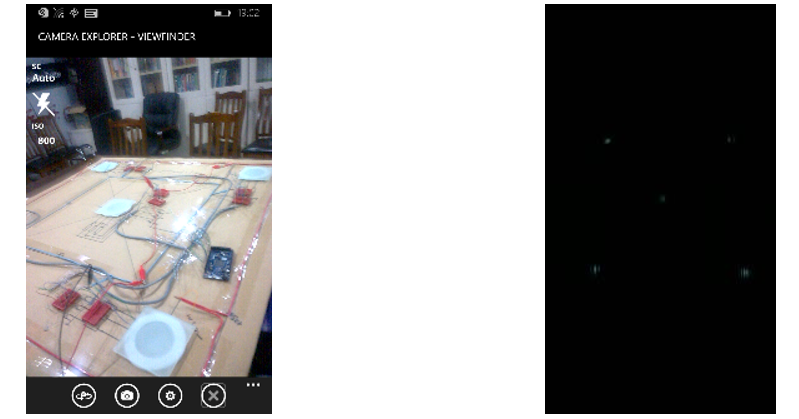
\includegraphics[width=0.8\linewidth]{Figure5.png}
	\caption{Camera App and a captured image showing the rolling shutter effect}
	\label{fig:subfig}
\end{figure}

\subsection*{4.3 Image Process Pipeline}
The image process pipeline receives a captured image from the camera, and apply image processing on it. We name the leds on the image \textit{transmitters}. We must determine the corresponding relationship between transmitters and physical LED beacons so that we can apply AoA localization. As we introduced above, we use frequency as the pairing key, and exploits rolling shutter effect to discover frequency on the captured image. So the image process pipeline exploits OpenCV to locate transmitters and their coordinates on the image and tagged them with frequencies based on the rolling shutter effect.

The pipeline's workflow is listed in Figure 6 below. We apply image processing methods 
\begin{figure}[h]
	\centering 
	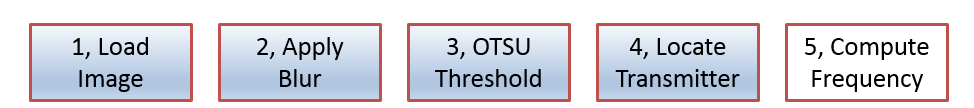
\includegraphics[width=0.8\linewidth]{Figure6.png}
	\caption{Workflow of the image processing pipeline}
	\label{fig:subfig}
\end{figure}


\subsection*{4.4 AoA}

\section*{5. Evaluation and Conclusion}

%----------------------------------------------------------------------------------------
%	BIBLIOGRAPHY
%----------------------------------------------------------------------------------------

\begin{thebibliography}{10}
	
\bibitem[1]{Radar00}
P.Bahl, V.N. Padmanabhan,
``Radar: An in-building RF-Based User Location and Tracking System.''
\textit{Proc. of IEEE INFOCOM}, volumn 2, pp. 775-784, 2000.

\bibitem[2]{Cricket04}
Nissanka Bodhi Priyantha,
``The Cricket Indoor Location System.''
\textit{ACM SIGCOMM},2004.

\bibitem[3]{Centaur12}
R.Nandakumar, K.K.Chintalapudi, and V.N.Padmanabhan,
``Centaur: Locating Devices in an Office Environment.''
\textit{ACM Mobicom},2012.

\bibitem[4]{Luxapose14}
Ye-Sheng Kuo, Pat Pannnuto,
``Luxapose: Indoor Positioning with Mobile Phones and Visible Light.''
\textit{ACM Mobicom},2014.

\bibitem[5]{Ubicarse14}
Swarun Kumar, Stephanie Gil, Dina Katabi, Daniela Rus,
``Accurate Indoor Localization with Zero Start-up Cost.''
\textit{ACM Mobicom},2014.


\bibitem[6]{google}
Googlers Talk Indoor Maps For 40 Minutes,
``http://www.webpronews.com/googlers-talk-\\indoor-maps-for-40-minutes-video-2013-05.''
\textit{}.

\bibitem[7]{Modellet14}
Liqun Li, Guobin Shen
``Experiencing and Handling the Diversity in Data Density and Environmental Locality in an Indoor Positioning Service''
\textit{ACM Mobicom},2014.

\bibitem[8]{NCE}
Microsoft
``https://github.com/Microsoft/camera-explorer''
\textit{}

\bibitem[9]{AoA}
M.C.Dean
``Bearings-Only Localization and Mapping.''
\textit{PhD thesis, Carnegie Mellon University},2005.


\end{thebibliography}

%----------------------------------------------------------------------------------------

\end{document}